\documentclass{beamer}

\usefonttheme{professionalfonts} % using non standard fonts for beamer
\usefonttheme{serif} % default family is serif

\usepackage{hyperref}
%\usepackage{minted}
\usepackage{animate}
\usepackage{graphicx}
\def\Put(#1,#2)#3{\leavevmode\makebox(0,0){\put(#1,#2){#3}}}
\usepackage{colortbl}
\usepackage{tikz}
\usepackage{amssymb}
\usepackage{enumerate}
\usepackage{arydshln}
\usepackage{algorithm}
\usepackage{algpseudocode}

\colorlet{lightred}{red!25}
\colorlet{lightgreen}{green!25}


\newcommand\blfootnote[1]{%

  \begingroup

  \renewcommand\thefootnote{}\footnote{#1}%

  \addtocounter{footnote}{-1}%

  \endgroup

}

\makeatletter

%%%%%%%%%%%%%%%%%%%%%%%%%%%%%% Textclass specific LaTeX commands.

 % this default might be overridden by plain title style

 \newcommand\makebeamertitle{\frame{\maketitle}}%

 % (ERT) argument for the TOC

 \AtBeginDocument{%

   \let\origtableofcontents=\tableofcontents

   \def\tableofcontents{\@ifnextchar[{\origtableofcontents}{\gobbletableofcontents}}

   \def\gobbletableofcontents#1{\origtableofcontents}

 }

%%%%%%%%%%%%%%%%%%%%%%%%%%%%%% User specified LaTeX commands.

\usetheme{Malmoe}

% or ...

\useoutertheme{infolines}

\addtobeamertemplate{headline}{}{\vskip2pt}

\setbeamercovered{transparent}

% or whatever (possibly just delete it)

\makeatother

\begin{document}
\title[PFLOCK report]{PFLOCK Report}
\author[AC]{Andres Calderon}
\institute[Spring'20]{University of California, Riverside}
\makebeamertitle
\newif\iflattersubsect

\AtBeginSection[] {
    \begin{frame}<beamer>
    \frametitle{Outline} 
    \tableofcontents[currentsection]  
    \end{frame}
    \lattersubsectfalse
}

\AtBeginSubsection[] {
    \begin{frame}<beamer>
    \frametitle{Outline} 
    \tableofcontents[currentsubsection]  
    \end{frame}
}

\begin{frame}{Problems with local quadtree settings...}
    \begin{itemize}
        \item Building the local quadtree at each partition was taking most of the time.
        \item The parameters of the quadtree were quite sensible.  Small changes lead to large quadtrees.
        \item It increses significantly the number of comparisons.
    \end{itemize}
\end{frame}

\begin{frame}{Altenative...}
    \begin{itemize}
        \item Using the JTS Quadtree library to build the local indexes (much more stable).
        \item As the JTS Quadtree does not allow to extract the leaves' MBRs let's use a regular grid to query the index.
        \item A regular grid is created at each partition and the number of cells is set by the user.
        \item If partition's size is less than a threshold it will run the index-based approach.
    \end{itemize}
\end{frame}

\begin{frame}{Global grids...}
    \centering
    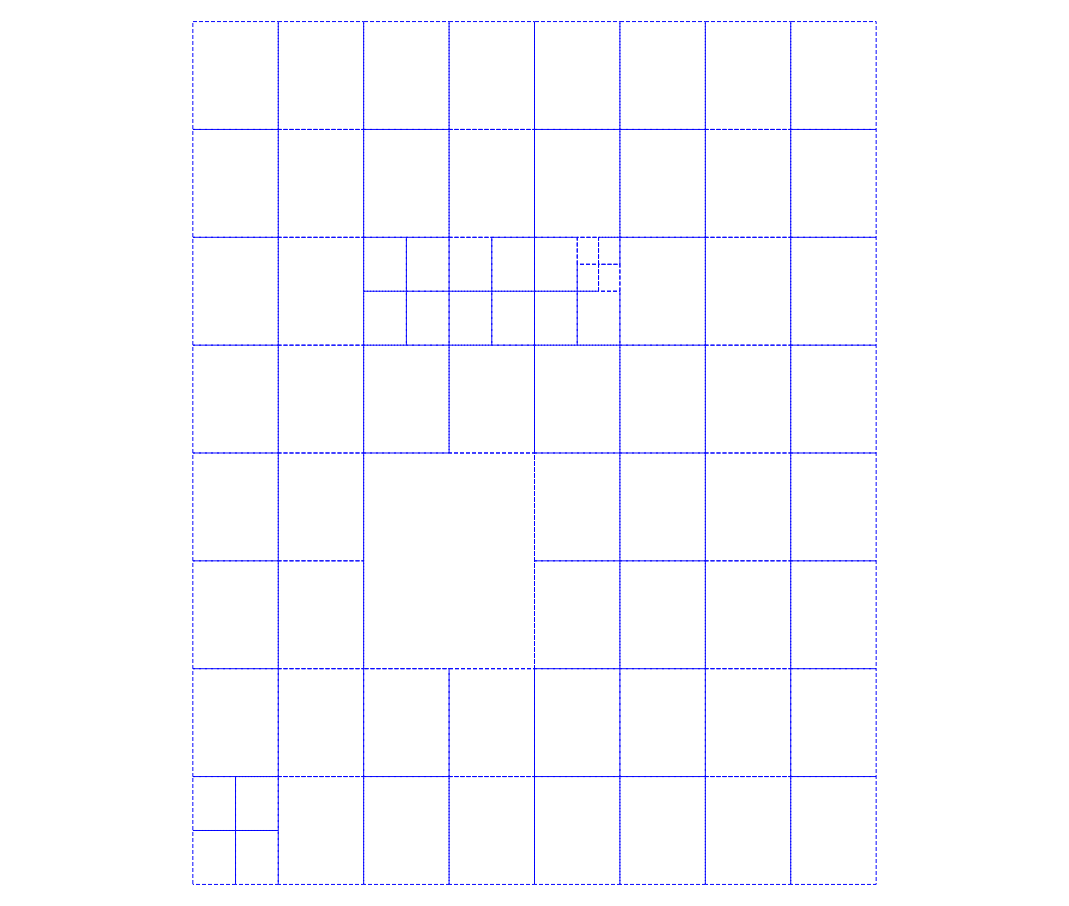
\includegraphics[width=0.75\textwidth]{figures/ggrids}
\end{frame}

\begin{frame}{Local grids...}
    \centering
    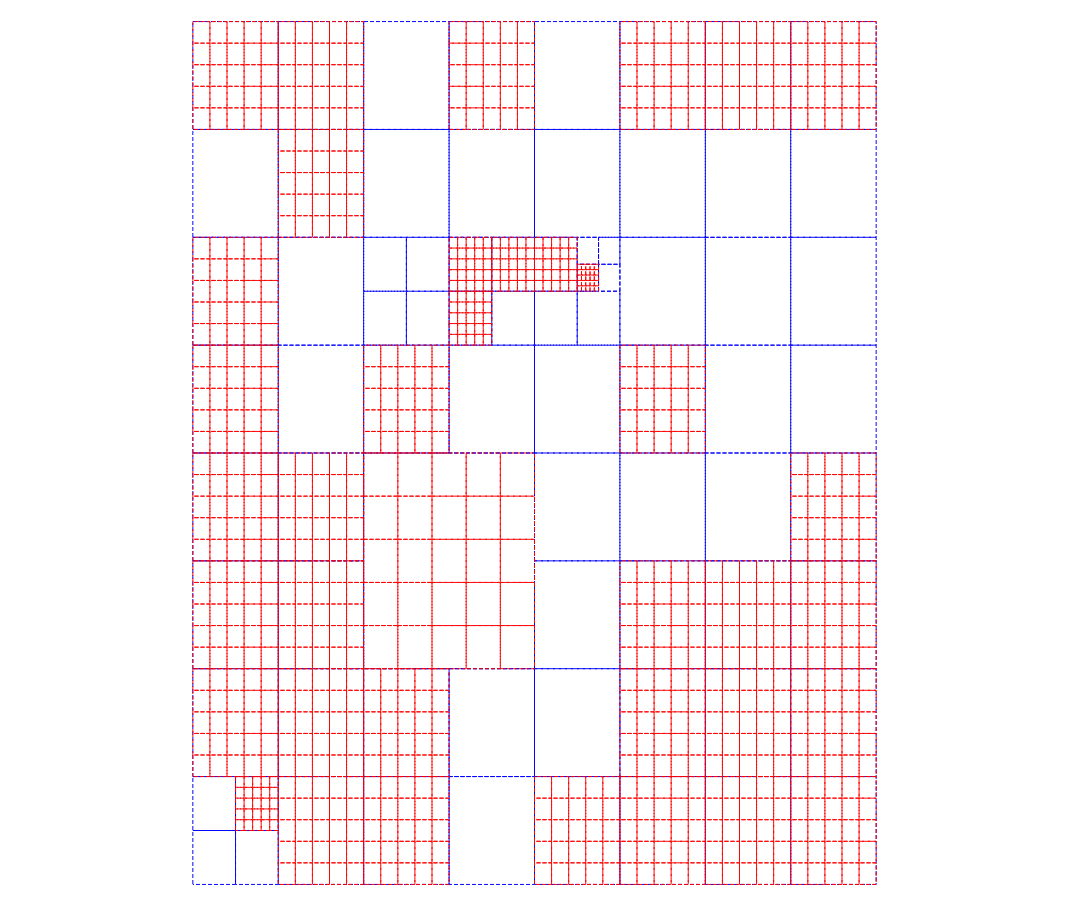
\includegraphics[width=0.75\textwidth]{figures/lgrids}
\end{frame}

\begin{frame}{Experiment setup...}
    \begin{itemize}
        \item Dataset: LA\_10K.
        \item $\mu=3$, varying values for $\varepsilon$ (from 10m to 30m).
        \item Running in local mode for now.
        \item Global partitioning: Quadtree, number of partitions: between 4 to 16.
        \item Average of 5 runs.
    \end{itemize}
\end{frame}

\begin{frame}{Results...}
    \centering
    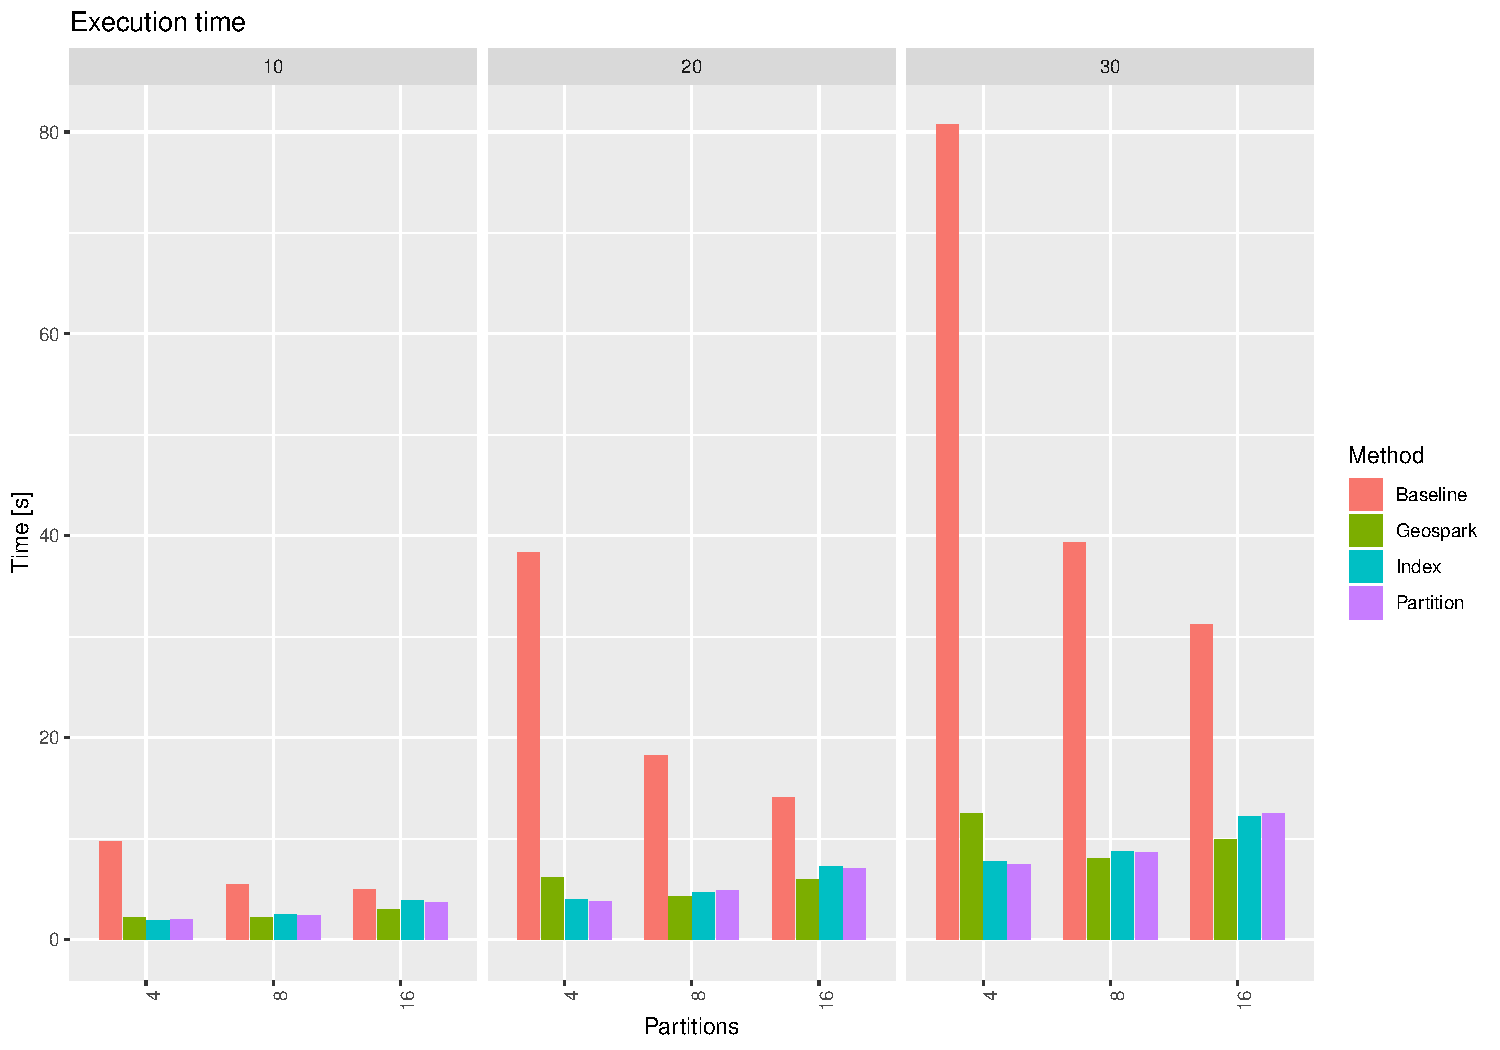
\includegraphics[width=0.85\textwidth]{figures/Test}
\end{frame}

\end{document}
